\section{Problem Statement}
\label{sec:problemStatement}

\begin{figure}[t]
\centering
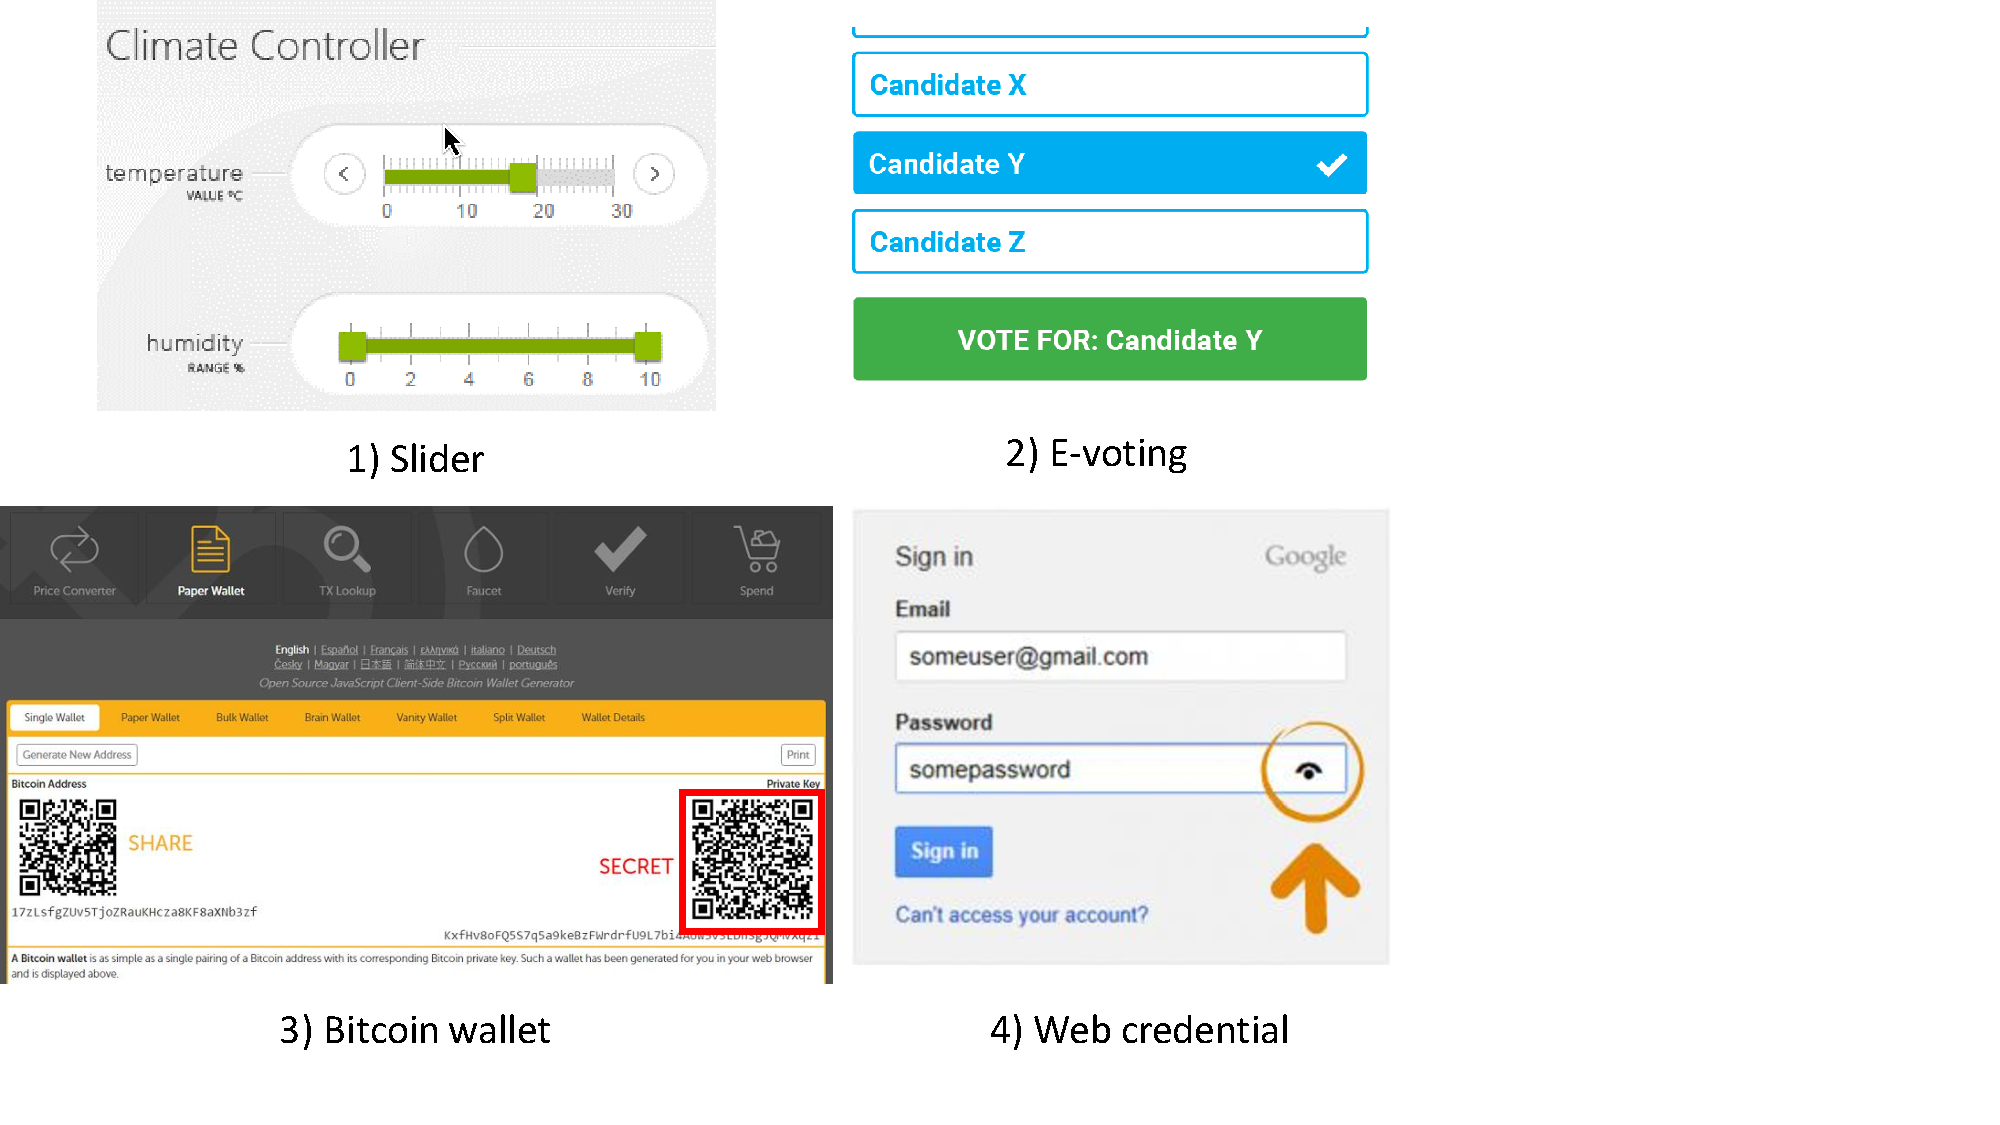
\includegraphics[trim={0 1cm 10cm 0}, clip, width=\linewidth]{motivation.pdf}
\caption{\textbf{\name motivating examples.} 1) Pointer based UI elements that sets parameters to remote safety-critical device, 2) E-voting where the voting privacy and integrity is critical, 3) Financial transactions such as bitcoin wallet that shows sensitive information such as the user's private key and 4) web appications that provide an option for the user to reveal credentials.}
\label{fig:motivation}
\centering
\end{figure}


\subsection{Motivation and Problem Statement}
Input integrity and privacy is a crucial problem when one assumes the attacker model where the attacker compromises host systems that include the hardware, the operating systems and all the installed applications. Such attacker model allows it not only to steal the sensitive information from the user but also manipulate them. Figure~\ref{fig:motivation} providers four such cases where the secrecy and the integrity of the input and output data is crucial. Based on these example we list 6 security properties that are provided by \name. We now discuss these security peroperties and corresponds them with the motivating example.

\begin{enumerate}
  \item \textbf{Input integrity.}
  \item \textbf{Input privacy.}
  \item \textbf{Output integrity.}
  \item \textbf{Output privacy.}
  \item \textbf{Activity integrity.}
  \item \textbf{Activity privacy.}
\end{enumerate}


The problem that we try to solve is the following

\begin{enumerate}
  \item Integrity of the input device data (keyboard, mouse\ldots) and corresponds it to the frame data (of the display device) in the presence of an attacker-controlled host system.
  \item Installation of a single device, no change in any of the existing system/software or human interactions.
\end{enumerate}

\subsection{Attacker Model}

We assume the highly adversarial scenario where the attacker compromises the host system completely (OS, installed applications and hardware). The attacker also controlled the network. We only assume that it is a PPT-attacker, so he can not break crypto. Figure~\ref{fig:approachOverview} depicts the attacker model.

We only assume that the monitor, keyboard, mouse and the \device are trusted. Which is not unrealistic. The monitor, keyboard, and mouse have hardly any complex hardware. The TCB is very small.

\myparagraph{Advantages}

\begin{enumerate}
  \item The \device does not need to know the formatting/template of the page. As the \device only looks to the current mouse position, the structure of the page is somewhat irrelevant (?).
\end{enumerate}

\subsection{Limitations of the Known Solutions}

Previous research works such as IntegriKey~\cite{IntegriKey} uses a low-TCB embedded device to introduce a second factor for input integrity. Fidelius~\cite{Fidelius} uses raspberry pi's and Intel SGX to create a secure channel between the keyboard and the display device. By doing so Fidelius provides secure input and secure display for character based input. We inspired from Fidelius to extend it even further to generic IO operations for wider range of UI elements. Note that extending input devices, such as from a keyboard to a mouse is not a trivial task. Moreover, \name achieves this in the absence of any TEE as the trust model of \name is significantly different. 




